% Soubory musí být v kódování, které je nastaveno v příkazu \usepackage[...]{inputenc}

\documentclass[%
%  draft,              % Testovací překlad
  12pt,               % Velikost základního písma je 12 bodů
  %a4paper,            % Formát papíru je A4
  t,                  % obsah slajdů nebude centrovaný, nýbrž budou začínat od hora
  aspectratio=1610,   % poměr stran bude 16:10 (všechny projektory v učebnách na Technické 12), další volby jsou 43, 149, 169, 54, 32.
%  oneside,            % Jednostranný tisk (výchozí)
%% Z následujicich voleb lze použít maximálně jednu:
%  dvipdfm              % výstup bude zpracován programem 'dvipdfm' do PDF
%  dvips                % výstup bude zpracován programem 'dvips' do PS
%  pdftex              % překlad bude proveden programem 'pdftex' do PDF (výchozí)
  unicode,            % Záložky a informace budou v kódování unicode
% Z následujících voleb lze použít jen jednu:
%english,            % originální jazyk je angličtina
czech,              % originální jazyk je čeština (výchozí)
%slovak,             % originální jazyk je slovenčina
]{beamer}              % Dokument třídy 'zpráva'
%\usepackage{etex}

\usepackage[utf8]    %  Kódování zdrojových souborů je v UTF-8
  {inputenc}          % Balíček pro nastavení kódování zdrojových souborů
\usepackage{graphicx} % Balíček 'graphicx' pro vkládání obrázků
                      % Nutné pro vložení log školy a fakulty

\usepackage[
  nohyperlinks        % Nebudou tvořeny hypertextové odkazy do seznamu zkratek
]{acronym}            % Balíček 'acronym' pro sazby zkratek a symbolů
                      % Nutné pro použití prostředí 'seznamzkratek' balíčku 'thesis'

%% Balíček hyperref je volán třídou beamer automaticky
%\usepackage[
%  breaklinks=true,    % Hypertextové odkazy mohou obsahovat zalomení řádku
%  hypertexnames=false % Názvy hypertextových odkazů budou tvořeny
%                      % nezávisle na názvech TeXu
%]{hyperref}            % Balíček 'hyperref' pro sazbu hypertextových odkazů
%                      % Nutné pro použití příkazu 'nastavenipdf' balíčku 'thesis'

%\usepackage{pdfpages} % Balíček umožňující vkládat stránky z PDF souborů
                      %% Nutné při vkládání titulních listů a zadání přímo
                      %% ve formátu PDF z informačního systému

\usepackage{cmap}     % Balíček cmap zajišťuje, že PDF vytvořené `pdflatexem' je
                      % plně "prohledávatelné" a "kopírovatelné"

\usepackage{upgreek}  % Balíček pro sazbu stojatých řeckých písmem
                      % např. stojaté pí: \uppi
                      % např. stojaté mí: \upmu (použitelné třeba v mikrometrech)
                      % pozor, grafická nekompatibilita s fonty typu Computer Modern!

%% Nastavení českého jazyka při sazbě v češtině.
\usepackage[czech]{babel}
%\usepackage{babel}             % Balíček pro sazbu různojazyčných dokumentů; kompilovat (pdf)latexem!
                    % převezme si z parametrů třídy správný jazyk
\usepackage{lmodern}  % vektorové fonty Latin Modern, nástupce původních Knuthových Computern Modern fontů
\usepackage{textcomp} % Dodatečné symboly
\usepackage[T1]{fontenc}  % Kódování fontu - mj. kvůli správným vzorům pro dělení slov

%\usepackage{amsmath}
\usepackage{booktabs}      % Balíček, který umožňuje v tabulce používat příkazy \toprule, \midrule, \bottomrule 


\usepackage[%
%% Z následujících voleb lze použít pouze jednu
% left,               % Rovnice a popisky plovoucich objektů budou %zarovnány vlevo
  center,             % Rovnice a popisky plovoucich objektů budou zarovnány na střed (vychozi)
%% Z následujících voleb lze použít pouze jednu
semestral            %  sazba zprávy semestrálního projektu
%bachelor            %  sazba bakalářské práce
%diploma             % sazba diplomové práce
%treatise            % sazba pojednání o dizertační práci
%%%%%%phd                 % sazba dizertační práce
]{thesis}             % Balíček pro sazbu studentských prací
                      % Musí být vložen až jako poslední, aby
                      % ostatní balíčky nepřepisovaly jeho příkazy

%%%%%%%%%%%%%%%%%%%%%%%%%%%%%%%%%%%%%%%%%%%%%%%%%%%%%%%%%%%%%%%%%
%%%%%%      Definice informací o dokumentu             %%%%%%%%%%
%%%%%%%%%%%%%%%%%%%%%%%%%%%%%%%%%%%%%%%%%%%%%%%%%%%%%%%%%%%%%%%%%


\autor[Bc.]{Péter}{Tóth}
\vedouci[Ing.]{Tomáš}{Urbanec }[Ph.D.]
\nazev{Název studentské práce}{Title of Student's Thesis}
%\oponent[doc.\ Mgr.]{Křestní}{Příjmení}[Ph.D.]
\oborstudia{Teleinformatika}{Teleinformatics}
\fakulta{Fakulta elektrotechniky a komunikačních technologií}{Faculty of Electrical Engineering and Communication}
\ustav{Ústav radioelektroniky}{Department of Radio Electronics}
\logofakulta[loga/FEKT_zkratka_barevne_PANTONE_CZ]{loga/UTKO_color_PANTONE_CZ}
\rok{2017}
\datum{19.\,12.\,2017} % Datum se uplatní pouze v prezentaci k obhajobě
\misto{Brno}
\abstrakt{Táto práce se zaobírá zpracováním přijatých signálů z amatérských družic NO-83 a NO-84 ParkinsonSat na nízké oběžné dráze (Low Earth Orbit – LEO) vysílajících telemetrické údaje v pásmu $70\,\mathrm{cm}$ vln. které jsou postiženy dopplerovským posuvem kmitočtu. Kvůli povaze oběžné dráhy a kmitočtu vysílání, přijatý signál je znatelně poškozen dopplerovským posuvem kmitočtu, který se musí kompenzovat pro pozdější potřeby demodulace.
}{This project work is dealing with processing of received radio signals of LEO satellites NO-83 and NO-84 ParkinsonSat transmitting in the 70--centimeter band. The nature of this kind of setup makes the received signal bearing a large amount of Doppler shift, which needs to be compensated in order to demodulate it.
}
\klicovaslova{korekce dopplerského posuvu, NO-83, BRICsat, NO-84, PSat, družice LEO, archiv dat TLE}
  {doppler shift correction, NO-83, BRICsat, NO-84, PSat, LEO satellites, TLE data archive}
\podekovanitext{Rád bych poděkoval vedoucímu diplomové práce panu Ing.~Tomášu Urbanci, Ph.D.\ za odborné vedení, konzultace, trpělivost a podnětné návrhy k~práci.}
  % do tohoto souboru doplňte údaje o sobě, o názvu práce...

%%%%%%%%%%%%%%%%%%%%%%%%%%%%%%%%%%%%%%%%%%%%%%%%%%%%%%%%%%%%%%%%%%%%%%%%

%%%%%%%%%%%%%%%%%%%%%%%%%%%%%%%%%%%%%%%%%%%%%%%%%%%%%%%%%%%%%%%%%%%%%%%%
%%%%%%     Nastavení polí ve Vlastnostech dokumentu PDF      %%%%%%%%%%%
%%%%%%%%%%%%%%%%%%%%%%%%%%%%%%%%%%%%%%%%%%%%%%%%%%%%%%%%%%%%%%%%%%%%%%%%
%% Při vloženém balíčku 'hyperref' lze použít příkaz '\nastavenipdf'
\nastavenipdf
%  Nastavení polí je možné provést také ručně příkazem:
\hypersetup{
  pdftitle={Telemetrický archiv družic},      % Pole 'Document Title'
  pdfauthor={Tóth Péter},     % Pole 'Author'
  pdfsubject={Semestrální projekt},                 % Pole 'Subject'
  pdfkeywords={korekce dopplerského posuvu, NO-83, BRICsat, NO-84, PSat, družice LEO, archiv datTLE}             % Pole 'Keywords'
}
%%%%%%%%%%%%%%%%%%%%%%%%%%%%%%%%%%%%%%%%%%%%%%%%%%%%%%%%%%%%%%%%%%%%%%%
\logohlavicka          % vytvoření zkraceného loga VUT FEKT (FEEC) v hlavičce slajdu, nechte odkomentované

\usetheme{VUT}         % barvy a rozložení prezentace odpovídající VUT FEKT
% alternativne lze pouzit jina berevna temata, napr. 
%\usetheme{Darmstadt} \usecolortheme{default2}
% ale bez zaruky

\begin{document}

% v pripade zakomentovani se zobrazi v pravem dolnim rohu slajdu klikatelne navigacni symboly 
\vypninavigacnisymboly

% snimek s titulni strankou vysazen bez hornich, dolnich a postranich list (volba plain),
% neni tak vysazen ani nadpis snimku
\vytvortitulku

%%%%%%%%%%%%%%%%%%%%%%%%%%%%%%%%%%%%%%%%%%%%%%%%%%%%%%%%%%%%%%%%%%%%%%%
% 1.snimek s cili (zadanim) prace
\begin{frame} 
  % nadpis snímku
  \frametitle{Telemetrický archiv družic}
  \begin{itemize}
    \item Umělé družice na nízké oběžné dráze
    \item Příjem radiového signálu družic
    \item Korekce doppleroského posuvu
  \end{itemize}
\end{frame}

%%%%%%%%%%%%%
\begin{frame} 
  \frametitle{Nízka oběžná dráha}

  % prostředí alertblok, které slouží pro zdůraznění informace
%  \begin{alertblock}{Pro práci je klíčový Eulerův vzorec}
%    $$\eul^{\jmag x}=\cos x + \jmag\sin x$$
%  \end{alertblock}


  \begin{block}{Proč používame?}
    Výhody a nevýhody.
  \end{block}

  \begin{alertblock}{Jak proti?}
    \begin{itemize}
      \item Python
      \item GNURadio
    \end{itemize}
  \end{alertblock}
\end{frame} 


%%%%%%%%%%%%%
\begin{frame} 
  \frametitle{Plošný spoj}
  
  \begin{columns}[T]                 % prostředí sloupce s umístěním nahoře
    \begin{column}{0.4\textwidth}    % první sloupec
      Obrázek znázorňuje model:\\[2ex]
      %
      \begin{itemize}
        \item Deska
        \item Součástky
        \item Signály
        \item Napájení
      \end{itemize}
    \end{column}
    %
    \begin{column}{0.6\textwidth}    % druhý sloupec
      \begin{figure}%  
        \centering
        \vspace{1cm}                % horizontální mezera
%        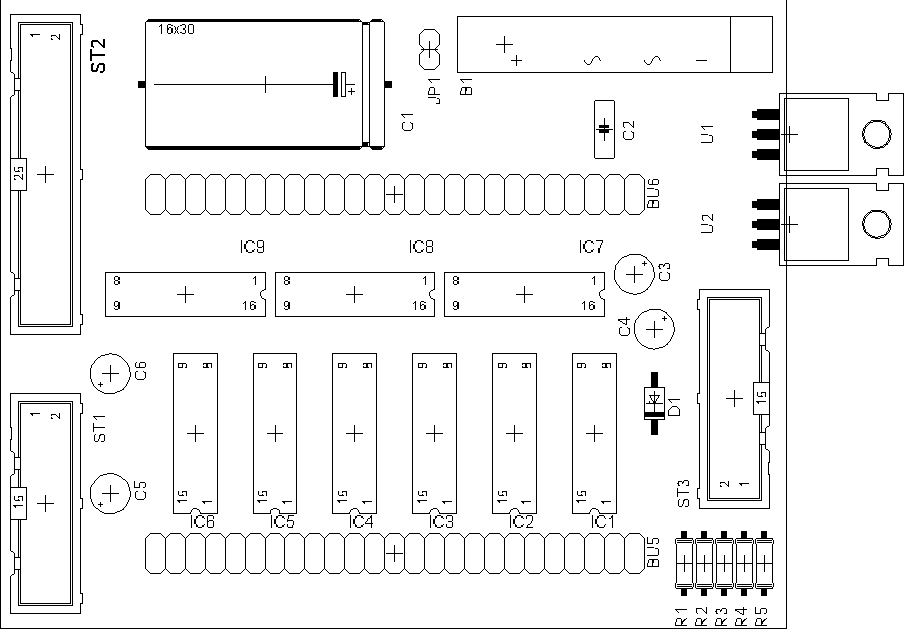
\includegraphics[width=0.8\columnwidth]{obrazky/soucastky}
        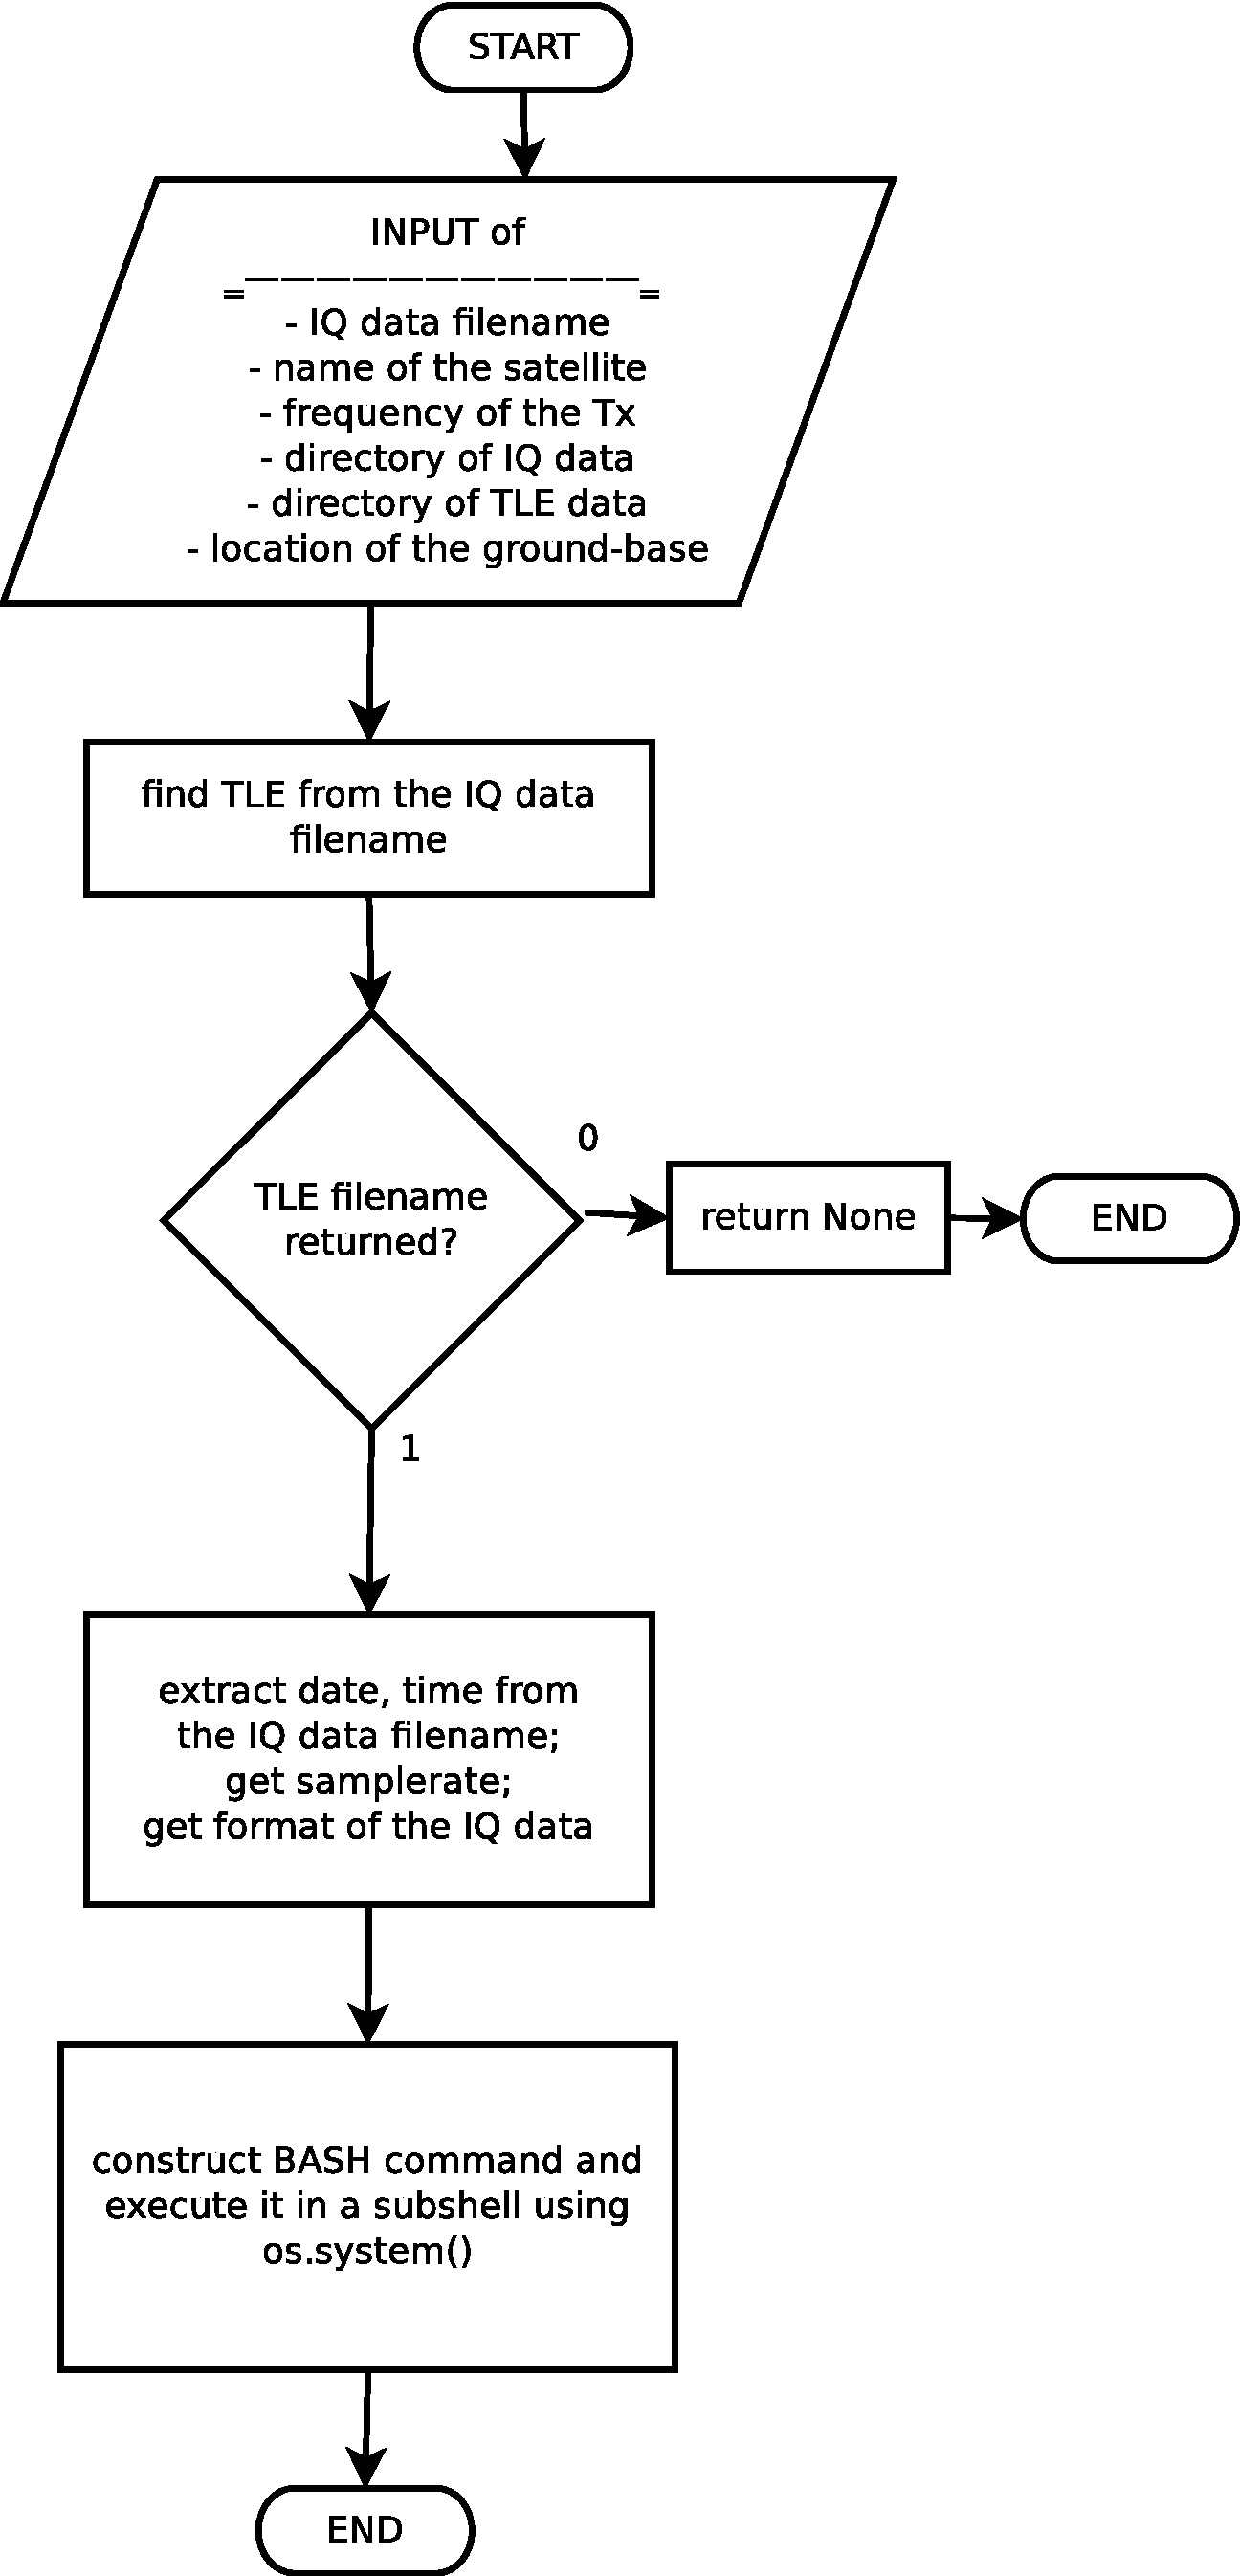
\includegraphics[width=0.8\columnwidth]{obrazky/get_undopplered}
        %lze vlozit popisek, ale povetsinou je to v prezentaci zbytecne
        %\caption{Popisek obrázku}%
        %\label{obr:ukazka}
      \end{figure}
    \end{column}
  \end{columns}                      % ukončení prostředí sloupce
\end{frame}


%%%%%%%%%%%%%
\begin{frame} 
  \frametitle{Výsledky}
  \vspace{1cm}
  \begin{table}[]
    \centering
    \caption{Výsledky měření mobilních sítí}
    \label{tab:tabulka}
      \begin{tabular}{lcc}
        \toprule
          Technologie  & Rychlost stahování [kB/s] & Rychlost nahrávání [kB/s] \\
        \midrule
          GPRS (2,5G)  & 7,2   & 3,6\\
          UMTS 3G     & 48     & 48\\
          HSPA (3,5G)  &  1\,706  &  720\\
          LTE (4G)     & 40\,750 & 10\,750\\
        \bottomrule                                       
      \end{tabular}
  \end{table}
\end{frame}


%%%%%%%%%%%%%
\begin{frame} 
  \frametitle{Závěr}
  \dots
\end{frame}


% podekovani
\begin{frame}[c] 
% bez nadpisu snimku
  \frametitle{\mbox{ }}
  \begin{center}
    {\Huge Děkuji za pozornost!}
  \end{center}
\end{frame}

\end{document}
